\let\negmedspace\undefined
\let\negthickspace\undefined
\documentclass[journal]{IEEEtran}
\usepackage[a5paper, margin=10mm, onecolumn]{geometry}
\usepackage{tfrupee}

\setlength{\headheight}{1cm}
\setlength{\headsep}{0mm}
\usepackage{gvv-book}
\usepackage{gvv}
\usepackage{cite}
\usepackage{amsmath,amssymb,amsfonts,amsthm}
\usepackage{algorithmic}
\usepackage{graphicx}
\usepackage{textcomp}
\usepackage{xcolor}
\usepackage{txfonts}
\usepackage{listings}
\usepackage{enumitem}
\usepackage{mathtools}
\usepackage{gensymb}
\usepackage{comment}
\usepackage[breaklinks=true]{hyperref}
\usepackage{tkz-euclide}
\def\inputGnumericTable{}
\usepackage[latin1]{inputenc}
\usepackage{color}
\usepackage{array}
\usepackage{longtable}
\usepackage{calc}
\usepackage{multirow}
\usepackage{hhline}
\usepackage{ifthen}
\usepackage{lscape}
\usepackage{booktabs}
\usepackage{tikz}
\usetikzlibrary{arrows.meta,angles,quotes}

\begin{document}

\bibliographystyle{IEEEtran}
\vspace{3cm}

\section*{\large\textbf{Problem}}

Find the coordinates of the foot of the perpendicular \( \vec{Q} \) drawn from \( \vec{P} = \myvec{3 \\ 2 \\ 1} \) to the plane \( \vec{N}^T \vec{x} = 1 \), where \( \vec{N} = \myvec{2 \\ -1 \\ 1} \). Also, find the distance \( \|\vec{P} - \vec{Q}\| \) and the image of the point \( \vec{P} \) treating the plane as a mirror.

\section*{\large\textbf{Solution}}

Let the point be:
\[
\vec{P} = \myvec{3 \\ 2 \\ 1}
\]

The plane is defined by:
\[
\vec{N}^T \vec{x} = 1
\quad \text{where} \quad
\vec{N} = \myvec{2 \\ -1 \\ 1}
\]

To find the foot of the perpendicular from \( \vec{P} \) to the plane, we use:
\[
\vec{Q} = \vec{P} - \frac{\vec{N}^T \vec{P} - 1}{\vec{N}^T \vec{N}} \vec{N}
\]

Compute:
\[
\vec{N}^T \vec{P} = \myvec{2 & -1 & 1} \myvec{3 \\ 2 \\ 1} = 6 - 2 + 1 = 5
\quad \Rightarrow \quad
\vec{N}^T \vec{P} - 1 = 4
\]
\[
\vec{N}^T \vec{N} = \myvec{2 & -1 & 1} \myvec{2 \\ -1 \\ 1} = 4 + 1 + 1 = 6
\]

So:
\[
\vec{Q} = \vec{P} - \frac{4}{6} \vec{N}
= \vec{P} - \frac{2}{3} \vec{N}
= \myvec{3 \\ 2 \\ 1} - \frac{2}{3} \myvec{2 \\ -1 \\ 1}
= \myvec{3 - \frac{4}{3} \\ 2 + \frac{2}{3} \\ 1 - \frac{2}{3}}
= \myvec{\frac{5}{3} \\ \frac{8}{3} \\ \frac{1}{3}}
\]

The distance is:
\[
\|\vec{P} - \vec{Q}\| = \left\| \frac{2}{3} \vec{N} \right\| = \frac{2}{3} \sqrt{6}
\]

The image of \( \vec{P} \) reflected across the plane is:
\[
\vec{R} = \vec{P} - 2 \cdot \frac{\vec{N}^T \vec{P} - 1}{\vec{N}^T \vec{N}} \vec{N}
= \vec{P} - \frac{4}{3} \vec{N}
= \myvec{3 \\ 2 \\ 1} - \frac{4}{3} \myvec{2 \\ -1 \\ 1}
= \myvec{3 - \frac{8}{3} \\ 2 + \frac{4}{3} \\ 1 - \frac{4}{3}}
= \myvec{\frac{1}{3} \\ \frac{10}{3} \\ -\frac{1}{3}}
\]

\section*{\large\textbf{Final Answer}}

\[
\boxed{
\text{Foot of perpendicular: } \vec{Q} = \myvec{\frac{5}{3} \\ \frac{8}{3} \\ \frac{1}{3}}
}
\quad
\boxed{
\text{Distance } \|\vec{P} - \vec{Q}\| = \frac{2}{3} \sqrt{6}
}
\quad
\boxed{
\text{Image of } \vec{P}: \myvec{\frac{1}{3} \\ \frac{10}{3} \\ -\frac{1}{3}}
}
\]






\section*{\large\textbf{Plot}}
\begin{figure}[H]
\centering
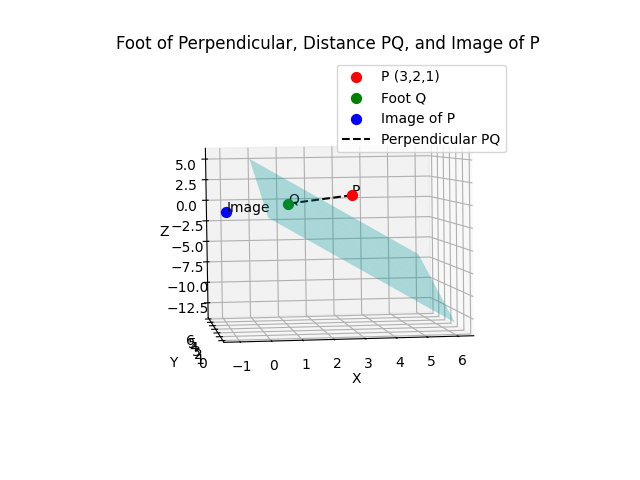
\includegraphics[width=1.1\linewidth]{Figs/Fig_1.png}
\caption{Point \( \vec{P} \) on the line and dividing \( \vec{A}\vec{B} \)}
\end{figure}







\end{document}





